\chapter{Database}
\label{chapter:database}

% setting up commands
\newcommand\scaleVal{0.71}
\newcommand\scaleContour{0.6}
\newcommand\scaleBlade{0.64}

The purpose of this chapter is to explain the generation of the database that will be used by the interpolation algorithm in Chapter~\ref{chapter:AI}. 
It starts explaining the domain of study and then it will define an appropriate strategy for increasing the overall convergence speed of the whole database.

This strategy can be seen as an additional \textit{acceleration} layer for the computation of an \textit{appropriate} initial guess, $\boldsymbol{x}_0$, used in the optimizer.

\begin{table}[!h]
    \caption{Domain boundaries and discretization.}
    \label{tab:domain}
    \begin{center}
        \renewcommand{\arraystretch}{2}
        \begin{tabularx}{0.6\textwidth} { 
            | >{\centering\arraybackslash}X 
            | >{\centering\arraybackslash}X 
            | >{\centering\arraybackslash}X 
            | >{\centering\arraybackslash}X | } 
            \hline
            \rowcolor{bluepoli!40}
            \textbf{Variable} & \textbf{Min} & \textbf{Max} & \textbf{Points} \\ [0.5ex] 
            \hline\hline
            $\alpha_1$ & $-50^{\circ}$ & $-20^{\circ}$ & 3 \\ [0.5ex]
            \hline
            $\alpha_2$ & $65^{\circ}$ & $72.5^{\circ}$ & 4 \\ [0.5ex]
            \hline
            $M_2$ & $0.4$ & $0.7$ & 3 \\ [0.5ex]
            \hline
            $Re$ & $6 \cdot 10^5$ & $6 \cdot 10^5$ & 1 \\ [0.5ex] 
            \hline
            $\frac{M_P}{M_{TE}}$ & $1.2$ & $1.4$ & 3 \\ [0.5ex]
            \hline
            $\frac{L_P}{L_{surf}}$ & $0.5$ & $0.6$ & 3 \\ [0.5ex]
            \hline
            $\frac{M_{LE}}{M_{TE}}\frac{M_2}{M_1}$ & $1.2$ & $1.8$ & 3 \\ [0.5ex]
            \hline
            $\frac{M_{PS}}{M_{TE}}\frac{M_2}{M_{1, ax}}$ & $0.8$ & $1.2$ & 3 \\ 
            \hline
        \end{tabularx}
    \end{center}
\end{table}

\section{Domain}

This study pertains to high-pressure turbine sections. 
The domain of study is presented in Table~\ref{tab:domain}.

Due to the \textbf{Reynolds indipendence} of the studied flow,the investigation has been carried out using a fixed Reynolds number value - $Re = 6 \cdot 10^5$. $\alpha_1$, $\alpha_2$, $M_2$, and $Re$ are physical quantities readily visualized within the problem setup.

The other four parameters, $\frac{M_{LE}}{M_{TE}}\frac{M_2}{M_1}$, $\frac{M_{PRESS}}{M_{TE}}\frac{M_2}{M_{1, ax}}$, $\frac{M_{PEAK}}{M_{TE}}$ and $\frac{L_{PEAK}}{L_{TOT}}$, 
constitutes engineering parameters that define the aerodynamic style properties. These parameters come out from numerours tests, aiming to identify values that both \textit{align with physics} and \textit{fit within blade capabilities}. 
These parameters are completelly arbitrary and are the most suitable for the intent of the present work.

The additional optimization strategy consists in linearizing the inner domain using outer domain points.
This will result in optimizing first the outer points of the domain, Table~\ref{tab:domain}, which will then provide a \textit{suitable} initial guess, $\boldsymbol{x}_0$, 
for the inner domain points. 

Figure~\ref{fig:linearInterpolation} shows the linear interpolation of the stagger angle, $\gamma$, with 
respect to the inlet flow angle, $\alpha_1$, and outlet flow angle, $\alpha_2$. 

\begin{figure}[H]
    \centering
    \includegraphics[scale=\scaleContour]{./images/staggerLinear.eps}
    \caption{Linear interpolation of the stagger angle, $\gamma$, with respect to $\alpha_1$ and $\alpha_2$ from the corner points in red.}
    \label{fig:linearInterpolation}
\end{figure}

This interpolation procedure is applied to all the blade parameters: starting from the 
camberline parameters and ending to the blade thickness parameters.

\subsection{Outer Points}

The computation of the corner points of the domain is the first step for the generation of the database. 
These points are the most time-consuming to converge, as the optimizer might start from an initial 
guess far from the optimal configuration.

Computing these corner points is critical, as it accelerates the computation of the inner points of the domain and increases the probability of optimizer convergence for inner points.

With the domain boundaries listed in Table~\ref{tab:domain}, \texttt{datablade} optimizes 128 blades to generate the corner points of the domain.

% The computation of the corner points is crucial because it allows to speed up the computation of the inner points of the domain as 
% well as increasing the probability of convergence of the optimizer for the inner points. 

% Given the domain boundaries showed in Table~\ref{tab:domain}, \texttt{datablade} has optimized 128 blades for the generation 
% of the corner points of the domain.

\subsection{Inner Points}

\begin{figure}[H]
    \centering
    \includegraphics[scale=\scaleContour]{./images/staggerComplete.eps}
    \caption{Complete $\gamma$ variation with respect to $\alpha_1$ \& $\alpha_2$. Corner points in red and inner points in black.}
    \label{fig:linearInterpolationFinal}
\end{figure}

% Once the generation of the corner points, the inner points are computed starting from a linear interpolation of the domain. 
% The linear interpolation example is showed in Figure~\ref{fig:linearInterpolation} which represents a first approximation of the 
% stagger angle, $\gamma$, variation with respect to the inlet flow angle, $\alpha_1$, and the outlet flow angle, $\alpha_2$.
% 
% From Table~\ref{tab:domain}, 2916 blades will be optimized from the inner points study.
% 
% Figure~\ref{fig:linearInterpolationFinal} shows the interpolated $\gamma$ with respect of $\alpha_1$ and $\alpha_2$ 
% after having computed the whole database points.

Once the corner points are generated, inner points are computed using linear interpolation. An example of linear interpolation is shown in Figure~\ref{fig:linearInterpolation}, which provides a preliminary estimation of the stagger angle, $\gamma$, variation based on the inlet flow angle, $\alpha_1$, and the outlet flow angle, $\alpha_2$.

According to Table~\ref{tab:domain}, 2916 blades will be optimized for the inner points study.

Figure~\ref{fig:linearInterpolationFinal} shows the interpolated $\gamma$ with respect to $\alpha_1$ and $\alpha_2$ after all database points have been computed.

\section{Optimized Data}

The database contains Kulfan's parameters for the definitions of the blade geometry.
% Hereafter there will be defined some of the main blades which are of interest for 
% a first database analysis. The database's blades can be subdivided in three categories:
Below, some key blades of interest for initial database analysis are defined. The database's blades are categorized as follows:

\begin{itemize}
    \item Blade configuration with \textbf{low error} on the loading distribution \textit{and} \textbf{low error} on the exit flow angle
    \item Blade configuration with \textbf{low error} on the loading distribution \textit{but} \textbf{high error} on the exit flow angle\footnote{In the present work it is considered a high exit flow angle error: $\Delta \alpha_1 > 1^{\circ}$.}.
    \item Blade configuration with \textbf{high error} on the loading distribution \textit{and} \textbf{high error} on the exit flow angle 
\end{itemize}

% Table~\ref{tab:database} defines the whole database after optimization.
Table~\ref{tab:database} defines the complete database after optimization.

\begin{table}[H]  
    \centering
    \renewcommand{\arraystretch}{2}
    \caption{Data properties inside the optimized database.}
    \label{tab:database}
    \begin{tabular}{| l c c c c c c c |}
        \hline
                                       & $\boldsymbol{count}$ & $\boldsymbol{\mu}$ & $\boldsymbol{\sigma}$ & $\boldsymbol{min}$ & $\boldsymbol{25\%}$ & $\boldsymbol{75\%}$ & $\boldsymbol{max}$ \\ \hline\hline
        $\boldsymbol{cost}$            & $2916$               & $0.018399$         & $0.006787$            & $0.005445$         & $0.013499$          & $0.021949$          & $0.049249$         \\ \hline
        $\boldsymbol{\Delta \alpha_2}$ & $2916$               & $0.965338^\circ$   & $0.542963^\circ$      & $0.000366^\circ$   & $0.472465^\circ$    & $1.382774^\circ$    & $2.377860^\circ$   \\ \hline
    \end{tabular}
\end{table}

% Table~\ref{tab:database} presents an acceptable mean value over $cost$ and $\Delta \alpha_2$. It is important to notice 
% that the $75 \%$ of the database is has a cost below $2.75 \%$ which tells that most of the blade 
% converge to the targeted aerodynamic style. This first analysis is very important because it 
% tells indirectly that few blades will be dropped off from the machine learning analysis.

% Another important result from Table~\ref{tab:database} is that the machine learning algorithm has to 
% work also on the correction of the exit flow angle, $\alpha_2$. This because more than $25 \%$ of the 
% database features an exit flow angle error, $\Delta \alpha_2$, above $1^{\circ}$. 

% Figure~\ref{fig:goodBlade} represents the best results the optimizer can achieve.
% The computed load follows the target load and, at the same time, the exit angle error, 
% $\Delta \alpha_2$, is below an acceptable threshold of $1^\circ$. 

Table~\ref{tab:database} reveals an acceptable mean value for both $cost$ and $\Delta \alpha_2$. It is noteworthy that more than $75\%$ of the database has a cost below $2.75\%$, indicating that the majority of the blades converge toward the desired aerodynamic style. 
This initial analysis is crucial as it indirectly suggests that only a few blades will be excluded from the machine learning analysis.

Another important observation from Table~\ref{tab:database} is that the machine learning algorithm must also address the correction of the exit flow angle, $\alpha_2$. 
This is necessary because over $25\%$ of the database exhibits an exit flow angle error, $\Delta \alpha_2$, exceeding $1^{\circ}$.

Figure~\ref{fig:goodBlade} showcases the best results achievable by the optimizer. 
The computed load adheres to the target load, while maintaining an exit angle error, $\Delta \alpha_2$, below an acceptable threshold of $1^\circ$. 

\begin{figure}[H]
    \centering
    \hspace*{-0.6cm}
    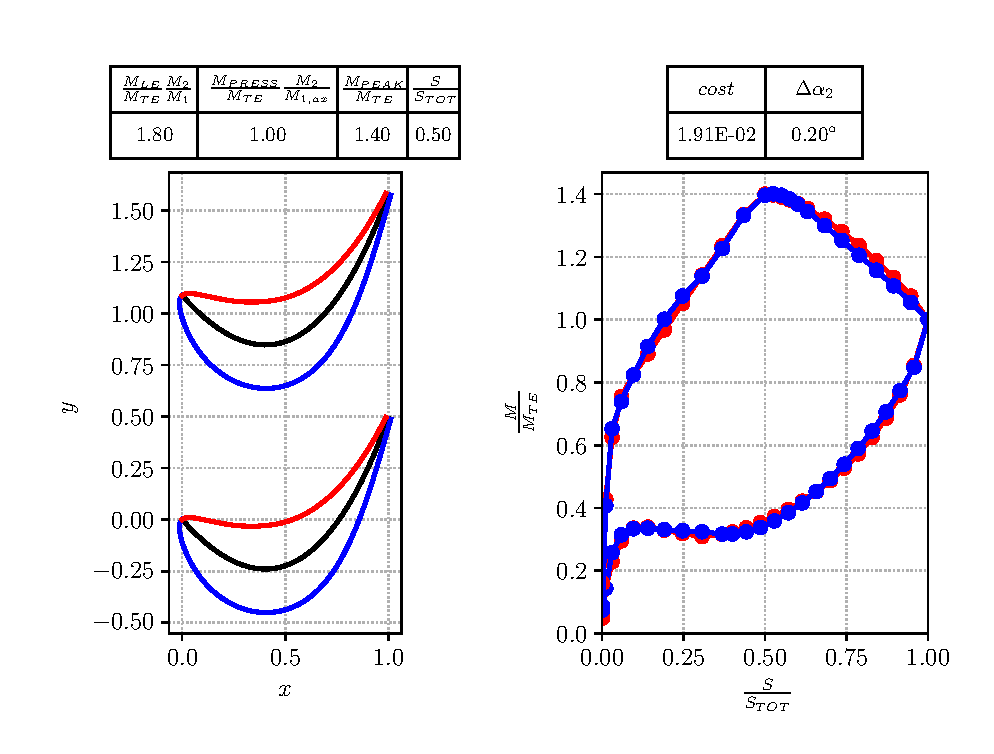
\includegraphics[scale=\scaleBlade]{./images/bladeVal0305.eps}
    \caption{Blade with good performances on the load distribution and on the exit angle error.}
    \label{fig:goodBlade}
\end{figure}

% Due to physics and the optimization algorithm, not every optimized blade follows 
% the target load distribution and has a low exit angle error at the same time. 
% 
% Figure~\ref{fig:badBlade} represents a \textit{poor-performing} blade. This blade will not be used inside the machine learning algorithm. 
% The reason of its esclusion is related to the high exit angle error and the non-acceptable error between the computed load and the target load.

Due to physical constraints and the optimization algorithm, not every optimized blade simultaneously achieves the desired loading distribution and a low exit angle error. 

Figure~\ref{fig:badBlade} represents a \textit{poor-performing} blade. Such blades are excluded from the machine learning analysis. 
The exclusion is due to the high exit angle error and the unacceptable discrepancy between the computed load and the target load.

\begin{figure}[H]
    \centering
    \hspace*{-0.6cm}
    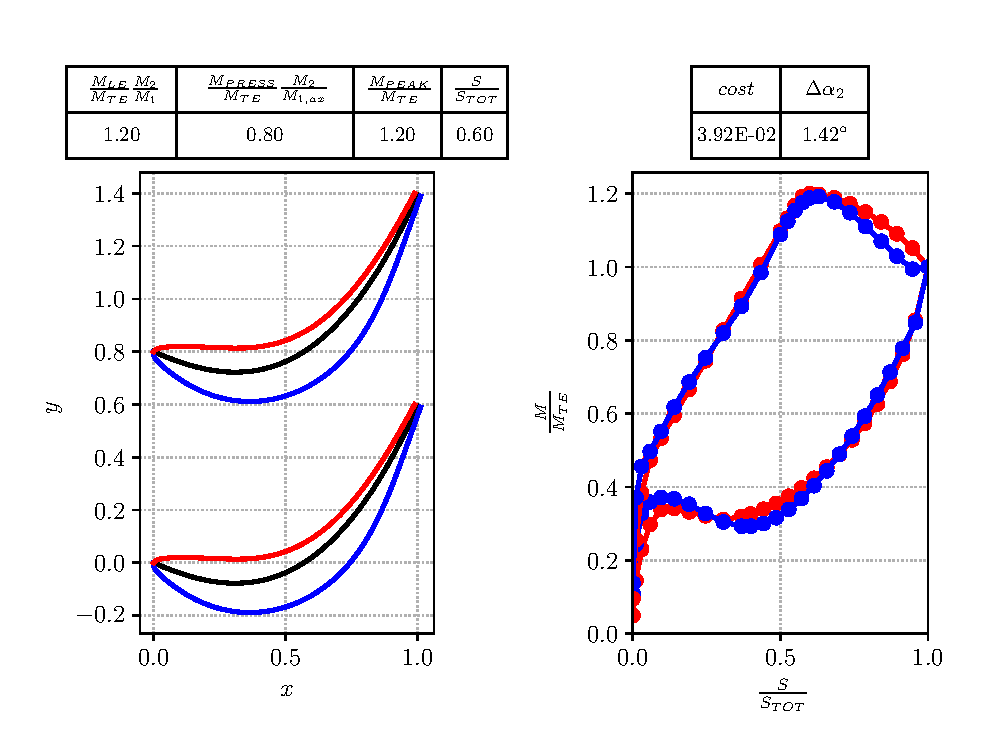
\includegraphics[scale=\scaleBlade]{./images/bladeVal1962.eps}
    \caption{Blade with poor performances on the load distribution and on the exit angle error.}
    \label{fig:badBlade}
\end{figure}

% These blades do not have a good impact on the database because they do not \textit{follow}
% appropriately the loading distribution. The main problem on these blades is related to the 
% loading distribution error. If a blade presents a high error on loading distribution, the 
% information it provides are not of any help inside the design space of study: this 
% because the blade represents something which has not any correlation with the desidered aerodynamic style.
% 
% Figure~\ref{fig:midBlade} shows an acceptable blade. Even though it has a high error on the exit flow angle this error can be fixed by the machine learning algorithm which will 
% \textit{displace} the interpolated field in order to have a good fit over the exit flow angle. 
% As it will be shown in Chapter~\ref{chapter:AI}, the exit flow 
% angle error can be corrected using an appropriate machine learning network. This 
% error can be seen as an information on the exit angle behavior for defined region of the design space.

These blades do not contribute effectively to the database because they do not appropriately match the loading distribution. 
The primary issue with these blades is the loading distribution error. If a blade exhibits a substantial error in loading distribution, the information it provides holds no relevance within the studied design space. 
This is because the blade configuration lacks correlation with the desired aerodynamic style.

Figure~\ref{fig:midBlade} depicts an acceptable blade. Despite its elevated exit angle error, the machine learning algorithm can rectify this error by shifting the interpolated field to achieve a better fit for the exit angle. 
As Chapter~\ref{chapter:AI} will demonstrate, the exit angle error can be corrected using a suitable machine learning network. This error can be interpreted as an information about exit angle behavior within specific regions of the design space.

\begin{figure}[H]
    \centering 
    \hspace*{-0.6cm}
    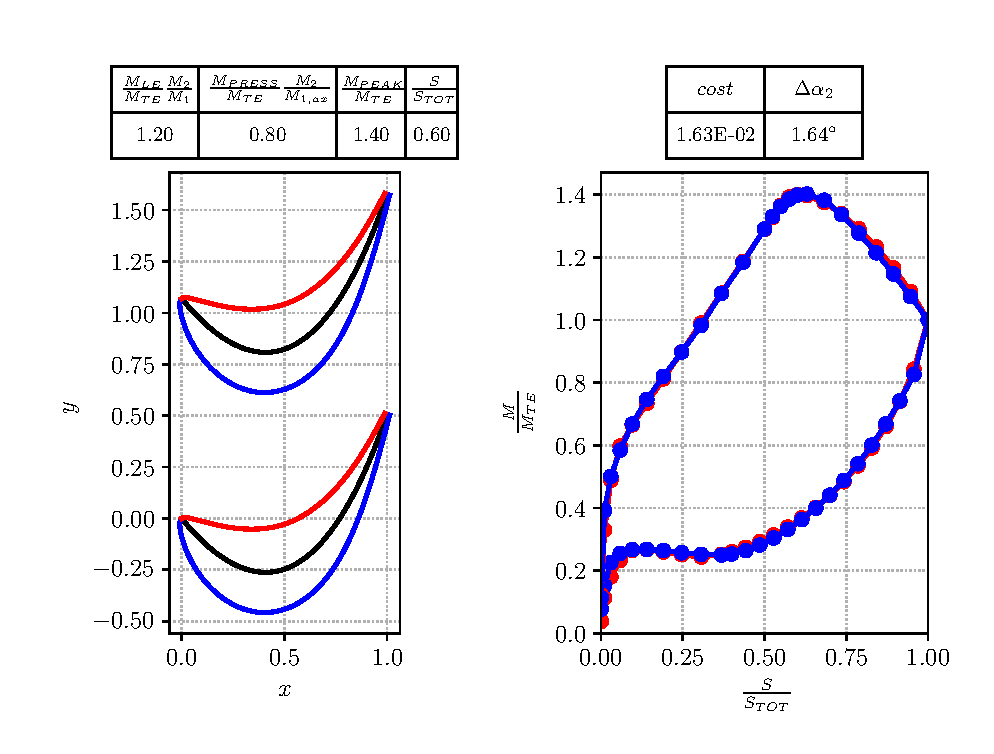
\includegraphics[scale=\scaleBlade]{./images/bladeVal0477.eps}
    \caption{Blade with good performances on the load distribution but low performance on the exit angle error.}
    \label{fig:midBlade}
\end{figure}

\subsection{Error Distribution}

As discussed in the previous sections, there are blades which present a significant error on the loading distribution, denoted by $RMSE$.
This error cannot be corrected by the machine learning algorithm under any circumstances; this is related by the 
fact that \textbf{bad input data} will inevitably lead to \textbf{bad output data}.
Blades falling into this category of \textit{unacceptable designs} are referred to as \textbf{unfeasible designs}.

% These configurations will be dropped off in order to give to the machine learning algorithm only useful data for 
% the interpolation. 
These particular configurations will be omitted to provide the machine learning algorithm only with useful data for interpolation.

Having introduced the concept of \textbf{unfeasible design} it is necessary to define the regions of the 
database where the error on the aerodynamic style can be considered \textit{not-acceptable}. 
In this study, the error in the aerodynamic style is considered \textit{not-acceptable} if it exceeds a cost threshold of $2.75\%$. 

\begin{figure}[H]
    \centering
    \includegraphics[scale=\scaleContour]{./images/costError1.eps}
    \caption{$cost$ distribution for $\alpha_1 = -50^{\circ}$, $\alpha_2 = 65^{\circ}$, $\frac{M_{PEAK}}{M_{TE}} = 1.4$, $\frac{S_{PEAK}}{S_{TOT}} = 0.5$ and $M_2 = 0.4$.}
    \label{fig:errorDistribution1}
\end{figure}

\begin{figure}[H]
    \centering
    \includegraphics[scale=\scaleContour]{./images/costError2.eps}
    \caption{$cost$ distribution for $\alpha_1 = -50^{\circ}$, $\alpha_2 = 65^{\circ}$, $\frac{M_{PEAK}}{M_{TE}} = 1.2$, $\frac{S_{PEAK}}{S_{TOT}} = 0.5$ and $M_2 = 0.4$.}
    \label{fig:errorDistribution2}
\end{figure}

Figure~\ref{fig:errorDistribution1} and Figure~\ref{fig:errorDistribution2} represent the two main regions where 
the error on the aerodynamic style is \textit{not-acceptable}.

\subsection{Filtering}

Although the data within the database can be processed by the machine learning algorithm, it is necessary to 
\textit{filter} the data in order to \textit{feed} only \textit{useful} entries to the interpolation algorithm - data 
which have significative relevance for the engineering purposes.

Table \ref{tab:filteredDatabase} presents the filtered database, representing a refined version after undergoing this data filtering process.

\begin{table}[H]  
    \centering
    \renewcommand{\arraystretch}{2}
    \caption{Filtered database.}
    \label{tab:filteredDatabase}
    \begin{tabular}{| l c c c c c c c |}
        \hline
                                       & $\boldsymbol{count}$ & $\boldsymbol{\mu}$ & $\boldsymbol{\sigma}$ & $\boldsymbol{min}$ & $\boldsymbol{25\%}$ & $\boldsymbol{75\%}$ & $\boldsymbol{max}$ \\ \hline\hline
        $\boldsymbol{cost}$            & $2787$               & $0.015233$         & $0.004874$            & $0.005554$         & $0.011249$          & $0.018777$          & $0.027483$         \\ \hline
        $\boldsymbol{\Delta \alpha_2}$ & $2787$               & $0.846587^\circ$   & $0.421034^\circ$      & $0.001229^\circ$   & $0.513713^\circ$    & $1.143698^\circ$    & $2.373522^\circ$   \\ \hline
    \end{tabular}
\end{table} 

In this revised dataset, the number of blades is slightly reduced compared to the original database. This reduction is attributed to the exclusion of certain blades due to their inadmissible errors in blade loading.

\begin{figure}[H]
    \centering
    \includegraphics[scale=\scaleContour]{./images/cost.eps}
    \caption{$cost$ function behavior in the domain.}
    \label{fig:cost}
\end{figure}

The \textbf{unfeasible designs} are concentrated at the \textit{boundaries} of the domain.
Figure~\ref{fig:cost} shows the cost function of a \textit{slice} of the domain. The data 
with a cost above $2.75\%$ have been dropped off. 

The filtering operation has been conducted \textit{only} over the $\boldsymbol{cost}$ properties of the blade.
Even though the $\boldsymbol{cost}$ relates the $RMSE$ and the $\Delta \alpha_2$, its value is dictated mainly by the $RMSE$.

Figure~\ref{fig:angleError} shows the error over the exit angle. The filtering operation are not made on the 
$\Delta \alpha_2$ domain.

\begin{figure}[H]
    \centering
    \includegraphics[scale=\scaleContour]{./images/angleError.eps}
    \caption{$\Delta \alpha_2$ function behavior in the domain.}
    \label{fig:angleError}
\end{figure}
